\documentclass{article}

\usepackage{tikz}
\usetikzlibrary{calc}

\usepackage[T1]{fontenc}
\usepackage[utf8]{inputenc}

\usepackage[ttdefault=true]{AnonymousPro}

\usepackage[a4paper, 
  textwidth=190mm,
  textheight=277mm
  ]{geometry}

\usepackage{fontspec}
% \setmainfont{QTCaligulatype}
%\setmainfont{QTBlackForest}

\newcommand{\kawalek}[4]{
  \begin{scope}[shift={#1}]
    \draw[dashed] (0,0) rectangle (8, 5);
    \node[text width=6cm, align=center, anchor=north] (gatunek) at (4, 3.8) {\setmainfont{QTCaligulatype}\bfseries\huge #2};
    \node[text width=6cm, align=center, anchor=north] (lacinka) at ($(gatunek.south)+(0, -0.2)$) {\slshape \ttfamily #3};
    \node[text width=6.5cm, align=center, anchor=north] (imie) at ($(lacinka.south)+(0, -0.3)$) {\bfseries\large\ttfamily #4};
    \draw[thick] (0.5, 0.5) rectangle (7.5, 4.5);
    \draw[dashed] (0.1, 0.1) rectangle (7.9, 4.9);
    \draw[ultra thick] (0.4, 0.4) rectangle (7.6, 4.6);
    \draw[thin, opacity=0.5] (0.45, 0.45) rectangle (7.55, 4.55);
  \end{scope}
}

\begin{document}

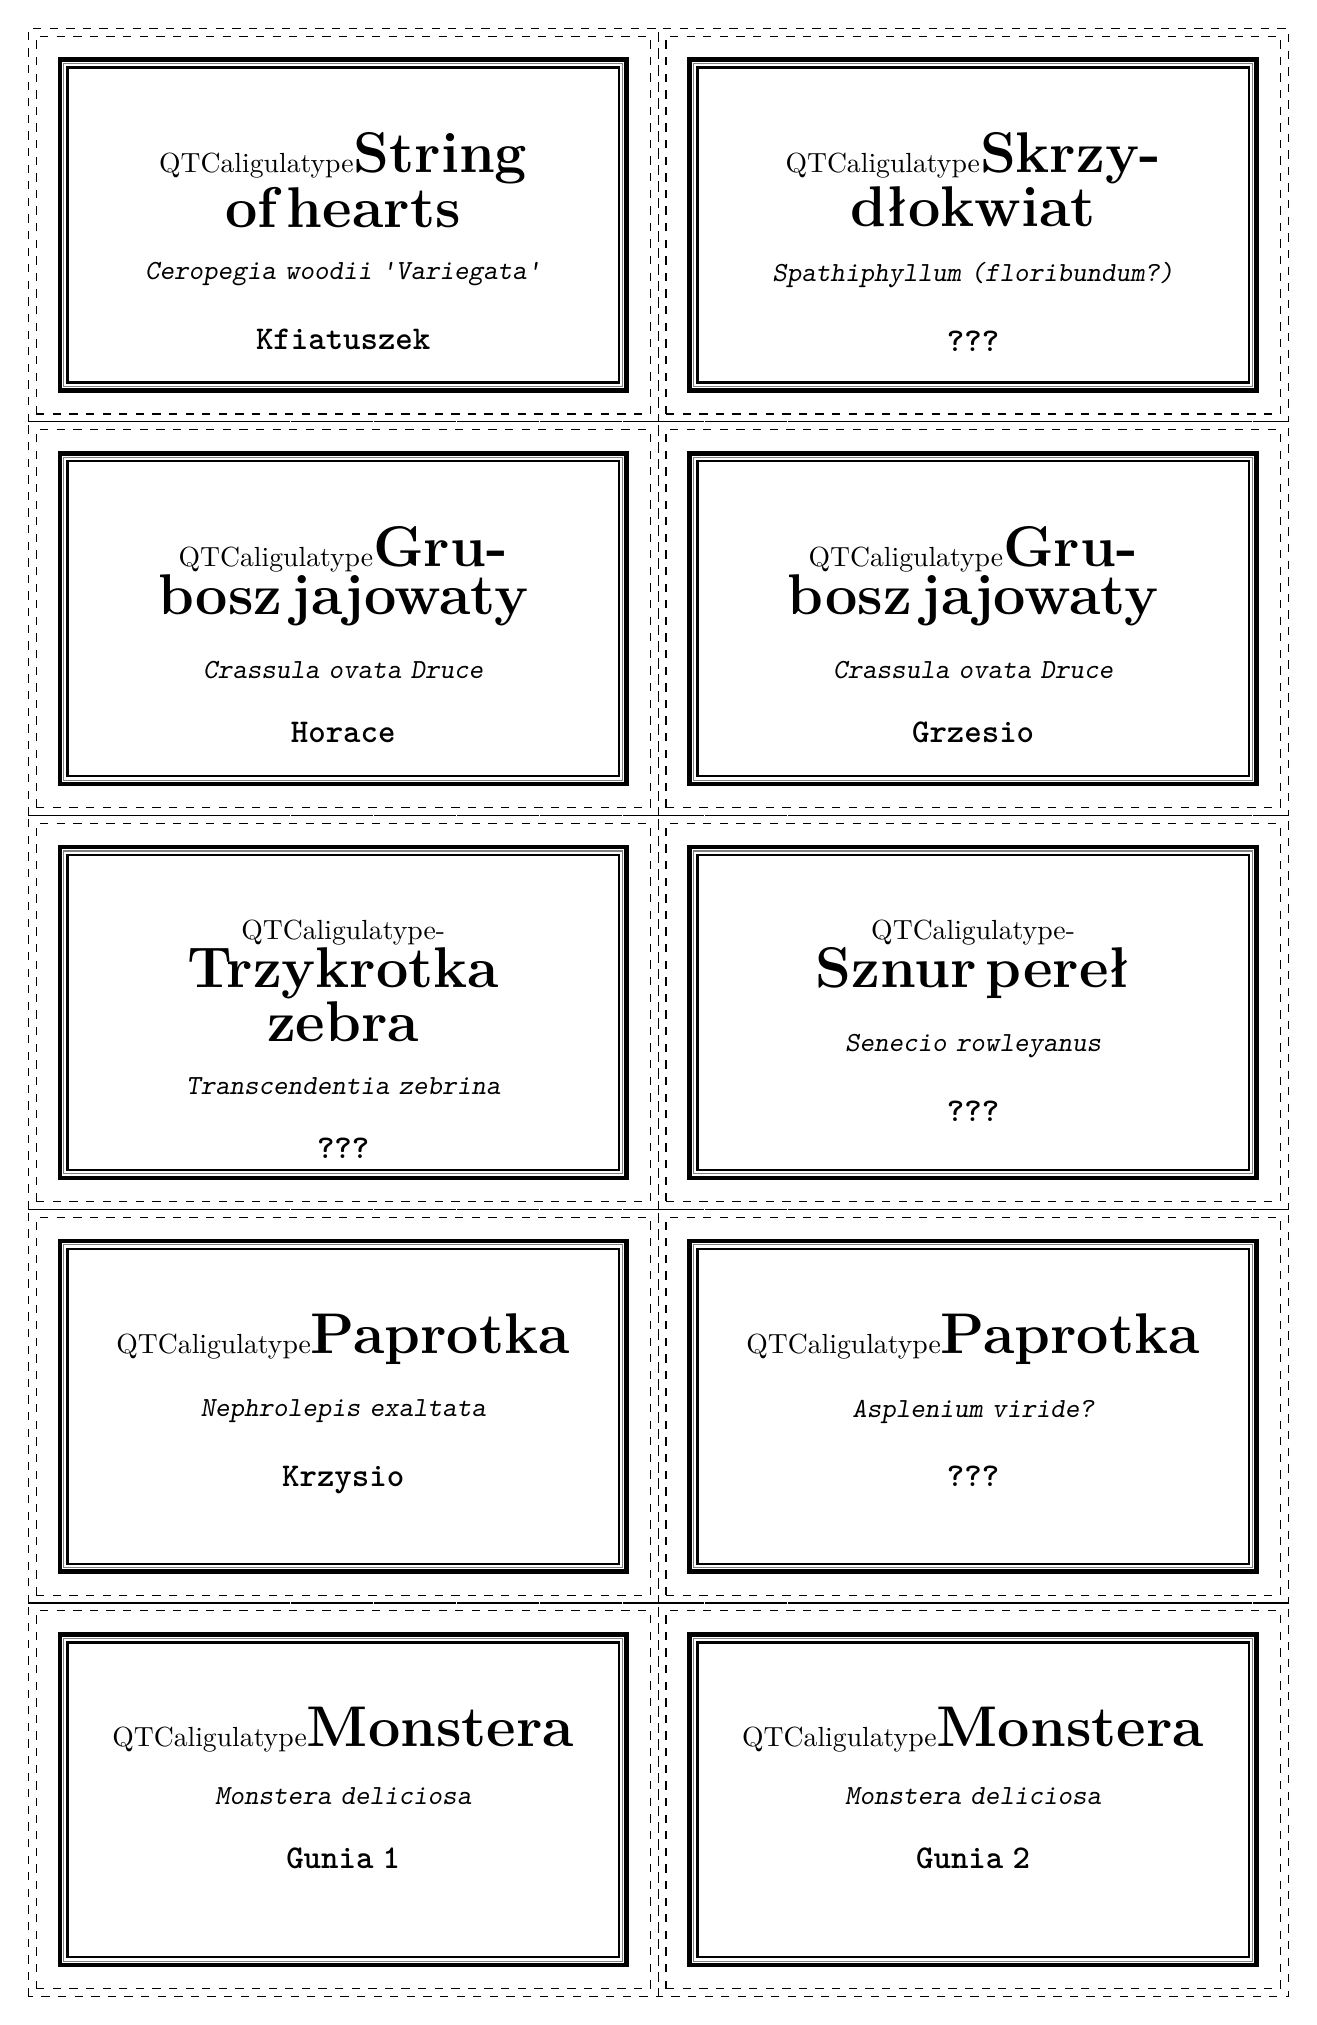
\begin{tikzpicture}
  \kawalek{(0,20)}{String of hearts}{Ceropegia woodii 'Variegata'}{Kfiatuszek}
  \kawalek{(8,20)}{Skrzydłokwiat}{Spathiphyllum (floribundum?)}{???}

  \kawalek{(8,15)}{Grubosz jajowaty}{Crassula ovata Druce}{Grzesio}
  \kawalek{(0,15)}{Grubosz jajowaty}{Crassula ovata Druce}{Horace}
  
  \kawalek{(0,10)}{Trzykrotka zebra}{Transcendentia zebrina}{???}
  \kawalek{(8,10)}{Sznur pereł}{Senecio rowleyanus}{???}

  \kawalek{(0,5)}{Paprotka}{Nephrolepis exaltata}{Krzysio}
  \kawalek{(8,5)}{Paprotka}{Asplenium viride?}{???}

  \kawalek{(0,0)}{Monstera}{Monstera deliciosa}{Gunia 1}
  \kawalek{(8,0)}{Monstera}{Monstera deliciosa}{Gunia 2}
\end{tikzpicture}

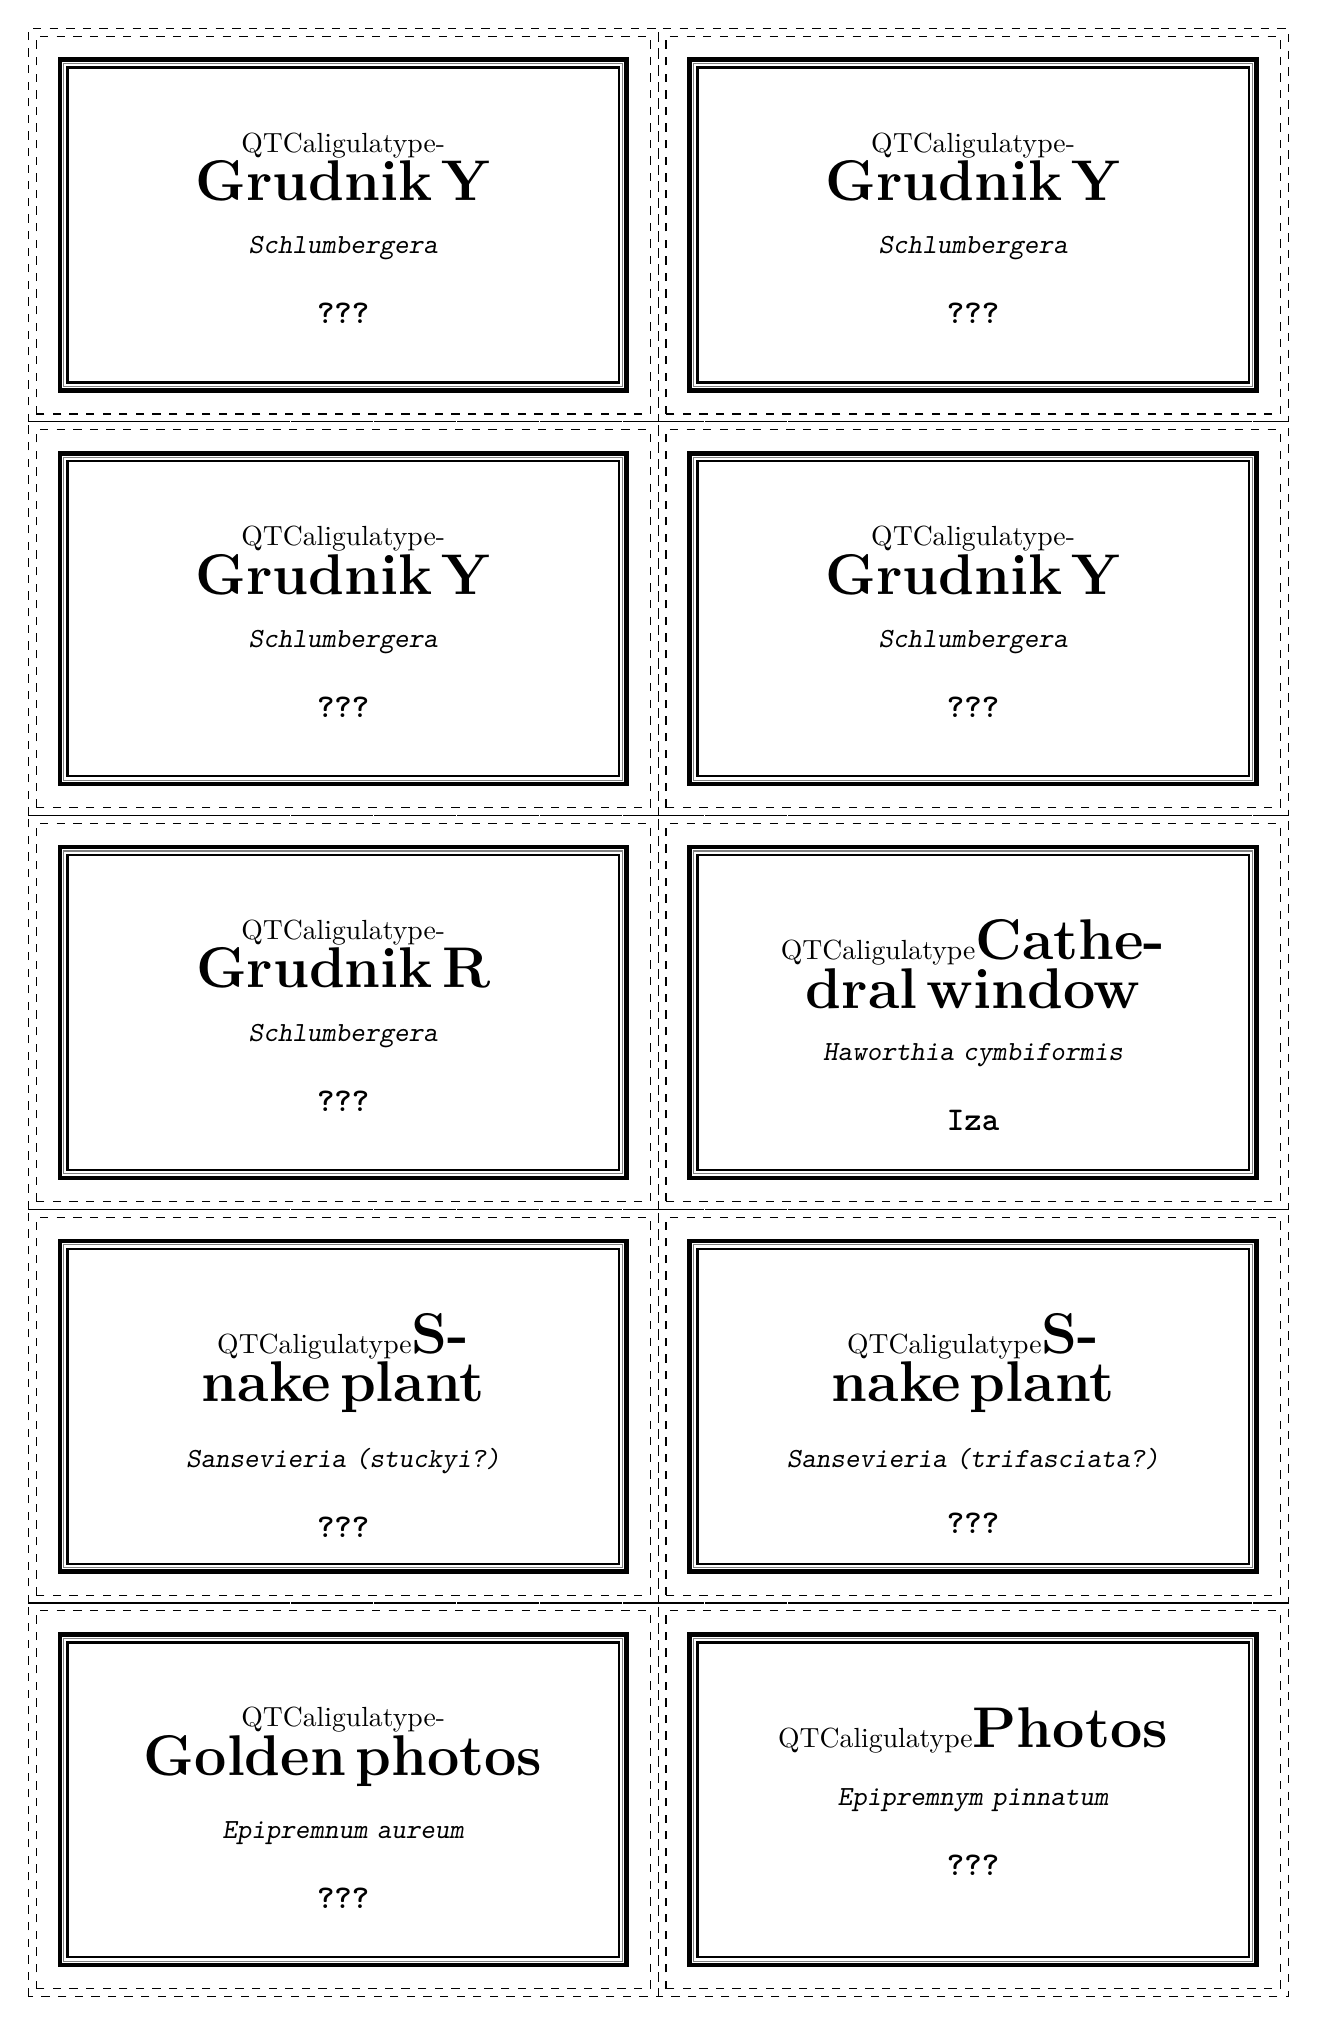
\begin{tikzpicture}
  \kawalek{(0,20)}{Grudnik Y}{Schlumbergera}{???}
  \kawalek{(8,20)}{Grudnik Y}{Schlumbergera}{???}

  \kawalek{(8,15)}{Grudnik Y}{Schlumbergera}{???}
  \kawalek{(0,15)}{Grudnik Y}{Schlumbergera}{???}
  
  \kawalek{(0,10)}{Grudnik R}{Schlumbergera}{???}
  \kawalek{(8,10)}{Cathedral window}{Haworthia cymbiformis}{Iza}

  \kawalek{(0,5)}{Snake plant}{Sansevieria (stuckyi?)}{???}
  \kawalek{(8,5)}{Snake plant}{Sansevieria (trifasciata?)}{???}

  \kawalek{(0,0)}{Golden photos}{Epipremnum aureum}{???}
  \kawalek{(8,0)}{Photos}{Epipremnym pinnatum}{???}
\end{tikzpicture}

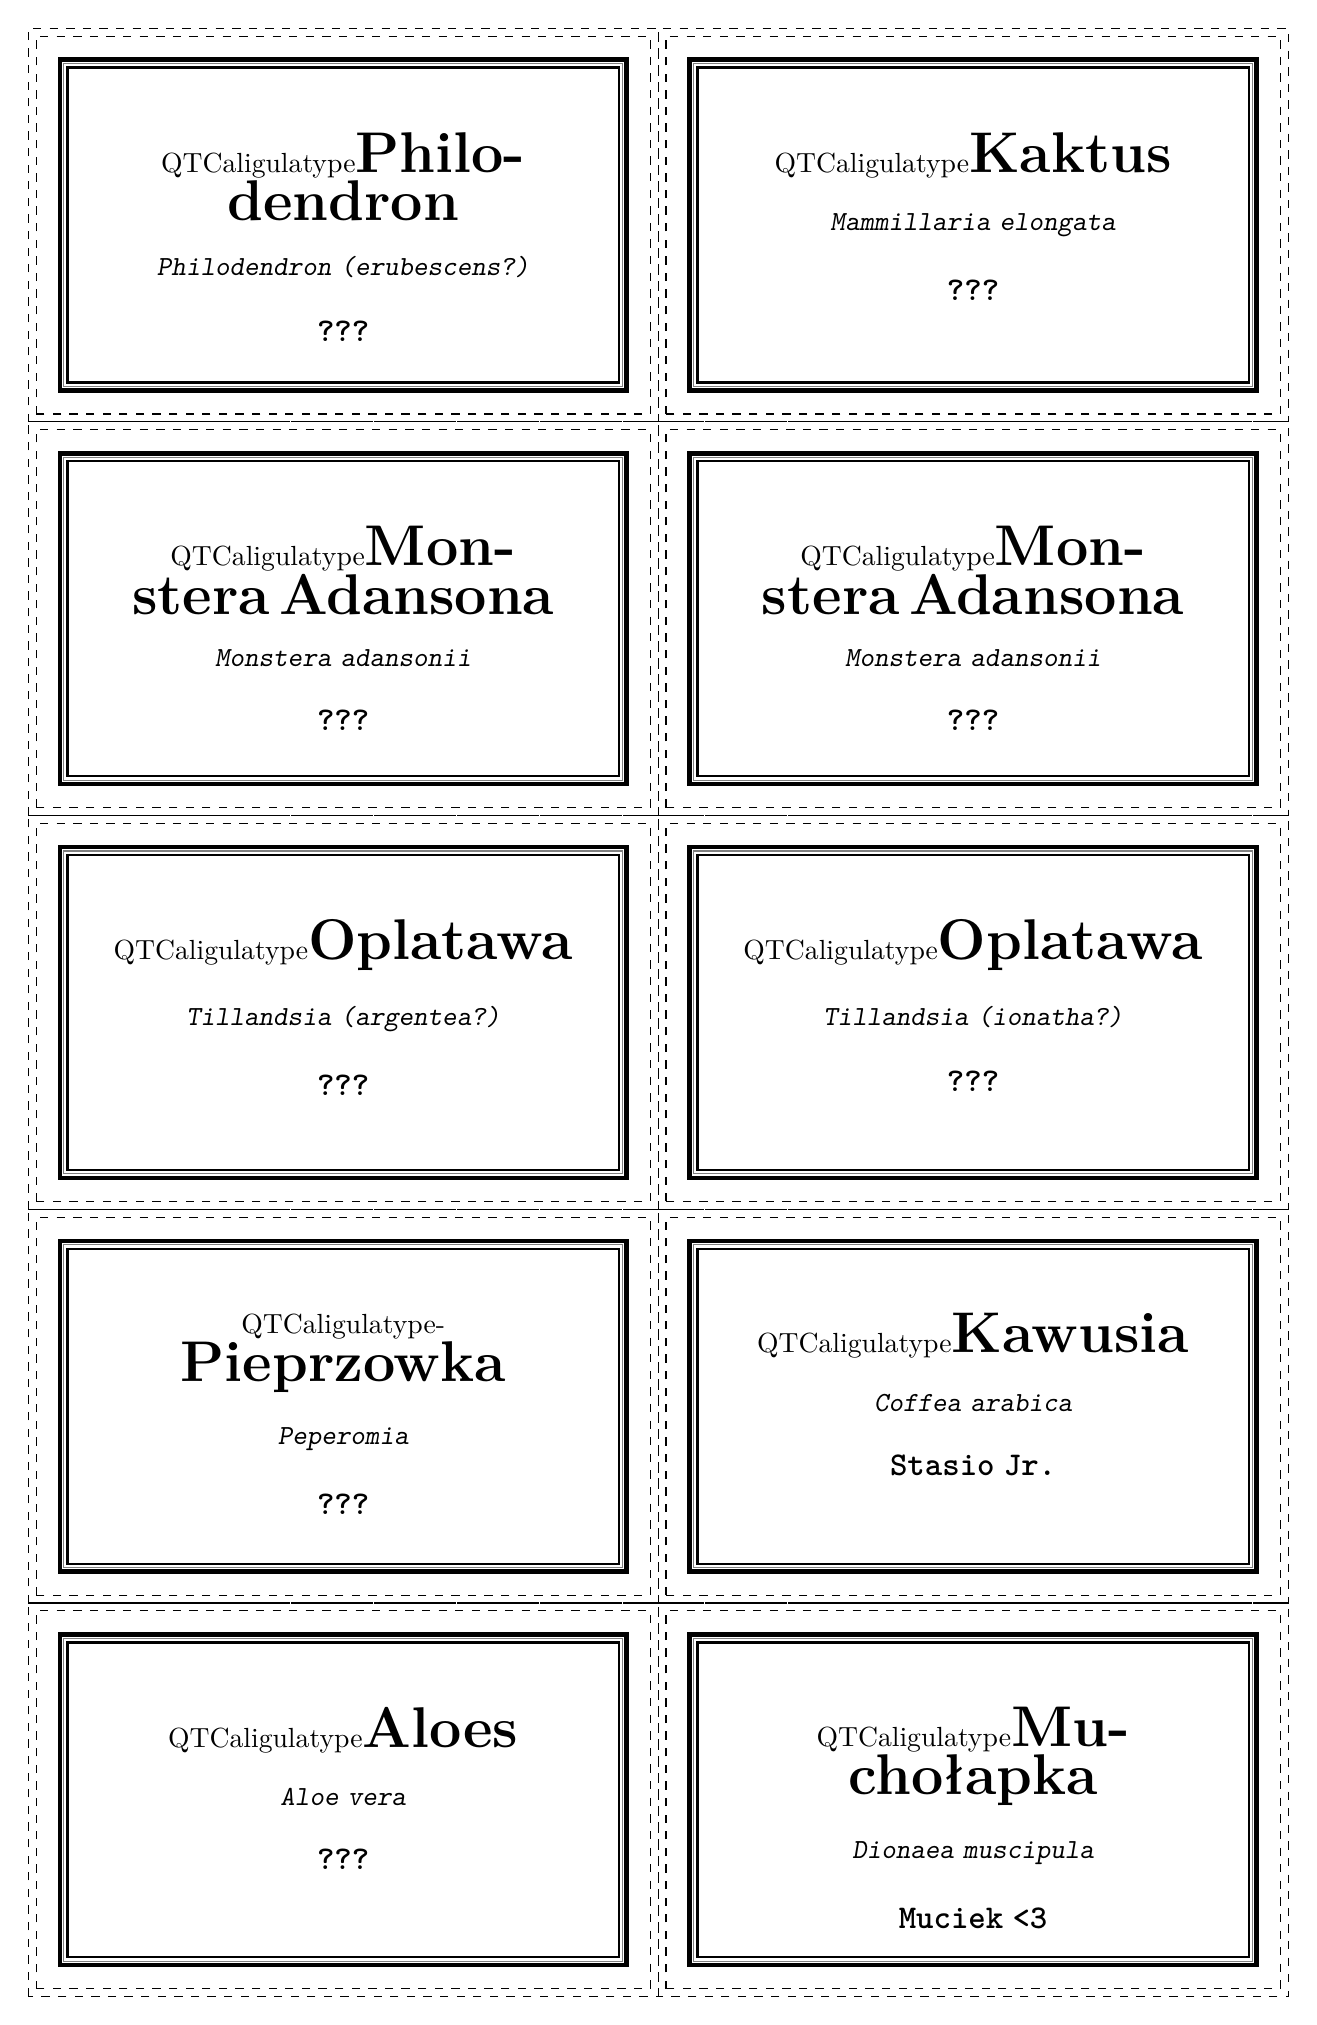
\begin{tikzpicture}
  \kawalek{(0,20)}{Philodendron}{Philodendron (erubescens?)}{???}
  \kawalek{(8,20)}{Kaktus}{Mammillaria elongata}{???}

  \kawalek{(8,15)}{Monstera Adansona}{Monstera adansonii}{???}
  \kawalek{(0,15)}{Monstera Adansona}{Monstera adansonii}{???}
  
  \kawalek{(0,10)}{Oplatawa}{Tillandsia (argentea?)}{???}
  \kawalek{(8,10)}{Oplatawa}{Tillandsia (ionatha?)}{???}

  \kawalek{(0,5)}{Pieprzowka}{Peperomia}{???}
  \kawalek{(8,5)}{Kawusia}{Coffea arabica}{Stasio Jr.}

  \kawalek{(0,0)}{Aloes}{Aloe vera}{???}
  \kawalek{(8,0)}{Muchołapka}{Dionaea muscipula}{Muciek <3}
\end{tikzpicture}

\end{document}
